\chapter{Supervised Learning}

\section{What is Supervised Learning}

Consider the example of recognizing handwritten digits, illustrated in the following figure.

\begin{figure}[h]
    \centering
    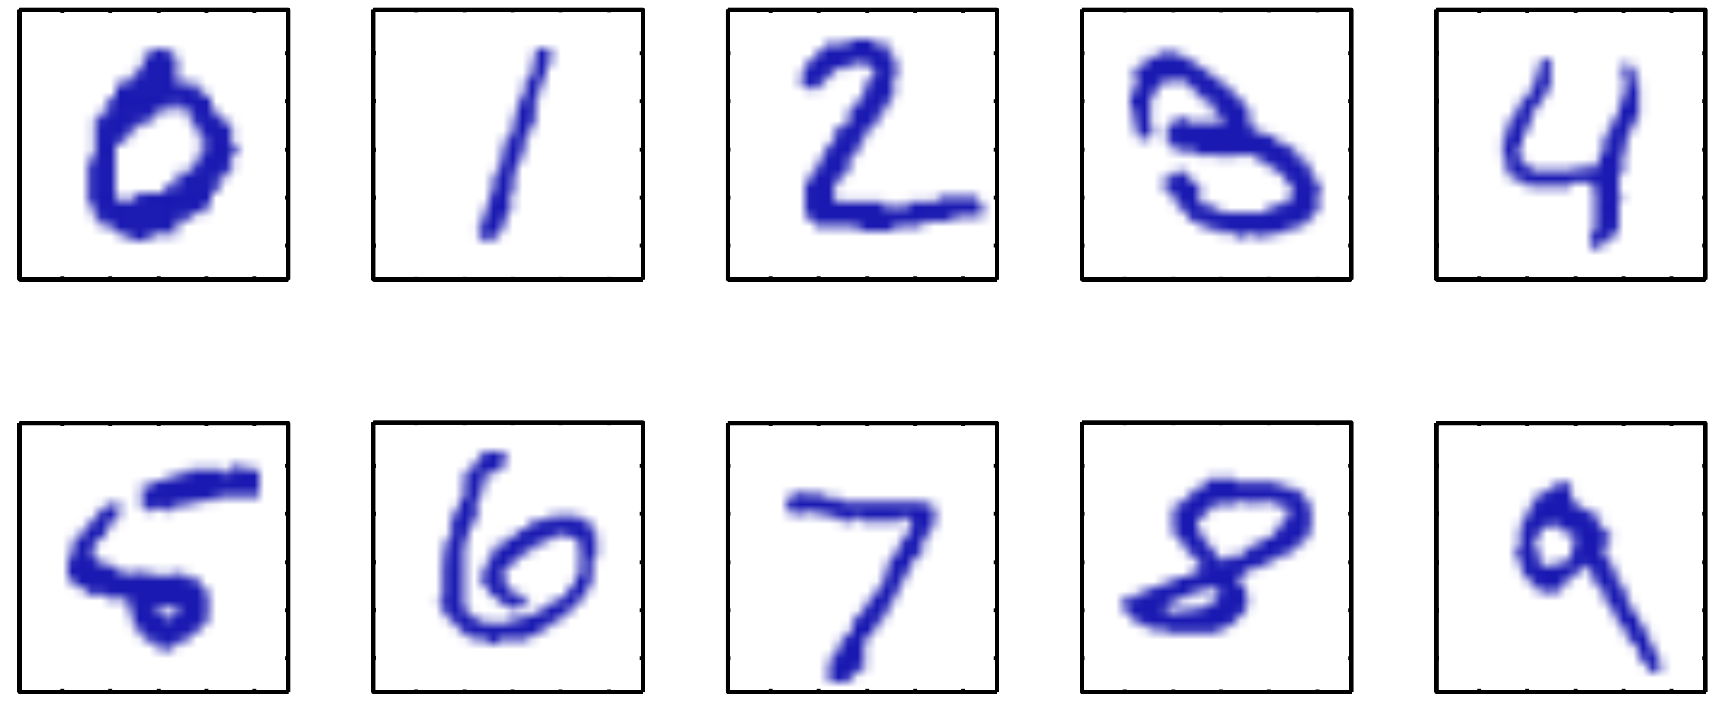
\includegraphics[scale=0.2]{chapter006/figures/fig001}
    \caption{handwritten digits}
    \label{handwritten digits}
\end{figure}

Each digit correspond to a $28 \times 28$ pixel image and so can be represented by a vector $x$ comprising $784$ real numbers. The goal is to build a machine that will take such a vector $x$ as input and that will produce the identity of the digit $0, ..., 9$ as the output.

In machine learning approach, given a large set of $N$ digits $\{x_1, ..., x_N\}$ called a \textit{training set} is used to tune the parameters of an adaptive model.

The categories of the digits in the training set are known in advance, typically by inspecting them individually and hand-labelling them.

We can express the category of a digit using \textit{target vector} $t$, which represents the identity of the corresponding digit. Note that there is one such target vector $t$ for each digit image $x$.

The result of running the machine algorithm can be expressed as a function $y(x)$ which takes a new digit image $x$ as input and that generates an output vector $y$, encoded in the same way as the target vectors.

The precise form of the function $y(x)$ is determined during the \textit{training phase}, also know as \textit{learning} phase, on the basic of the training data.

Once the model is trained it can then determine the identity of new digit images, which are said to comprise a \textit{test set}.

The ability to categorize new examples that differ from those used for training is known as \textit{generalization}.

For most practical applications, the original input variables are typically \textit{preprocessed} to transform them into some new space of variables where it is hoped, the pattern recognition problem will be easier to solve.

This pre-processing stage is sometimes also called \textit{feature extraction}. Note that new test data must be pre-processed using the same steps as the training data.

Pre-processing might also be performed in order to speed up computation or \textit{dimensionality reduction}.

Applications in which the training data comprises examples of the input vectors along with their corresponding target vectors are known as \textit{supervised learning} problems.

Assign each input vector to one of a finite number of \textbf{discrete categories}, are called \textit{classification}.

If the desired output consists of one or more continuous variables, then the task is called \textit{regression}.

\section{Polynomial Curve Fitting}

Suppose we observe a real-value input variable $x$ and we wish to use this observation to predict the value of a real-valued target variable $t$.

The data for this example is generated from the function $sin(2 \pi x)$ with random noise included in the target values.

Suppose that we are given a training set comprising $N$ observation of $x$. written $X \equiv (x_1, ..., x_N)^T$, together with corresponding observations of the values of $t$, denoted $T \equiv (t_1, ..., t_n)^T$

Our goal is to exploit this training set in order to make predictions of the value $\hat{t}$ of the target variable for some new value $\hat{x}$ of the input variables.

For the moment, we shall proceed rather informally and consider a simple approach based on curve fitting. In particular, we shall fit the data using a polynomial function of the form

\begin{equation}
    \label{Polynomial}
    y(x, \pmb{w}) = w_0 + w_1x + w_2x^2 + ... + w_Mx^M = \sum_{j=0}^Mw_jx^j
\end{equation}

where $M$ is the \textit{order} of the polynomial, and $x^j$ denotes $x$ raised to the power of $j$.

The polynomial coefficients $w_0, ..., w_M$ are collectively denoted by the vector $\pmb{w}$.

Note that, although the polynomial function $y(x, \pmb{w})$ is a nonlinear function of $x$, it is a linear function of the coefficients $\pmb{w}$. Functions, such as the polynomial, which are linear in the unknown parameters have important properties and are called \textit{linear models}.

The values of the coefficients will be determined by fitting the polynomial to the training data. This can be done by minimizing an \textit{error function} that measures the misfit between the function $y(x, \pmb{w})$, for any given value of $\pmb{w}$, and the training set data points.

One simple choice of error function, which is widely used, is given by the sum of the squares of the errors between the predictions $y(x_n, \pmb{w})$ for each data point $x_n$ and the corresponding target values $t_n$, so that we minimize

\section{Loss function}
\begin{equation}
    \label{Loss function}
    E(\pmb{w}) = \frac{1}{2} \sum_{n=1}^N \{y(x_n, \pmb{w})) - t_n \}^2
\end{equation}

where the factor of $\frac{1}{2}$ is included for later convenience.

We can solve the cure fitting problem by choosing the value of $\pmb{w}$ for which $E(\pmb{w})$ is as small as possible. Because the error function is a quadratic function of the coefficients $\pmb{w}$, its derivatives with respect to the coefficients will be linear in the elements of $\pmb{w}$, and so the minimization of the error function has a unique solution, denoted by $\pmb{w}*$, which can be found in closed form. The resulting polynomial is given by the function $y(x, \pmb{w}*)$.

There remains the problem of choosing the order $M$ of the polynomial.

We notice that the constant $(M = 0)$ and first order $(M = 1)$ polynomials give rather poor fits to the data and consequently rather poor representations of the training data.

The third order$(M = 3)$ polynomial seems to give the best fit to the data. When we go to a much higher order polynomial $(M = 9)$, we obtain an excellent fit to the training data. In fact, the polynomial passes exactly through each data point and $E(\pmb{w*}) = 0$. However, the fitted curve oscillates wildly and gives a very poor representation of the function $sin(2 \pi x)$. This latter behavior is known as \textbf{over-fitting}.




As we have noted earlier, the goal is to achieve good generalization by making accurate predictions for new data. We can obtain some quantitative insight into the dependence of the generalization performance on $M$ by considering a separate test comprising 100 data points generated using exactly the same procedure used to generate the training set points but with new choices for the random noise values included in the target values. For each choice of $M$, we can then evaluate the residual value of $E(\pmb{w*})$ for the training data, and we can also evaluate $\pmb{w*}$ for the test data set.


\begin{figure}[h]
    \centering
    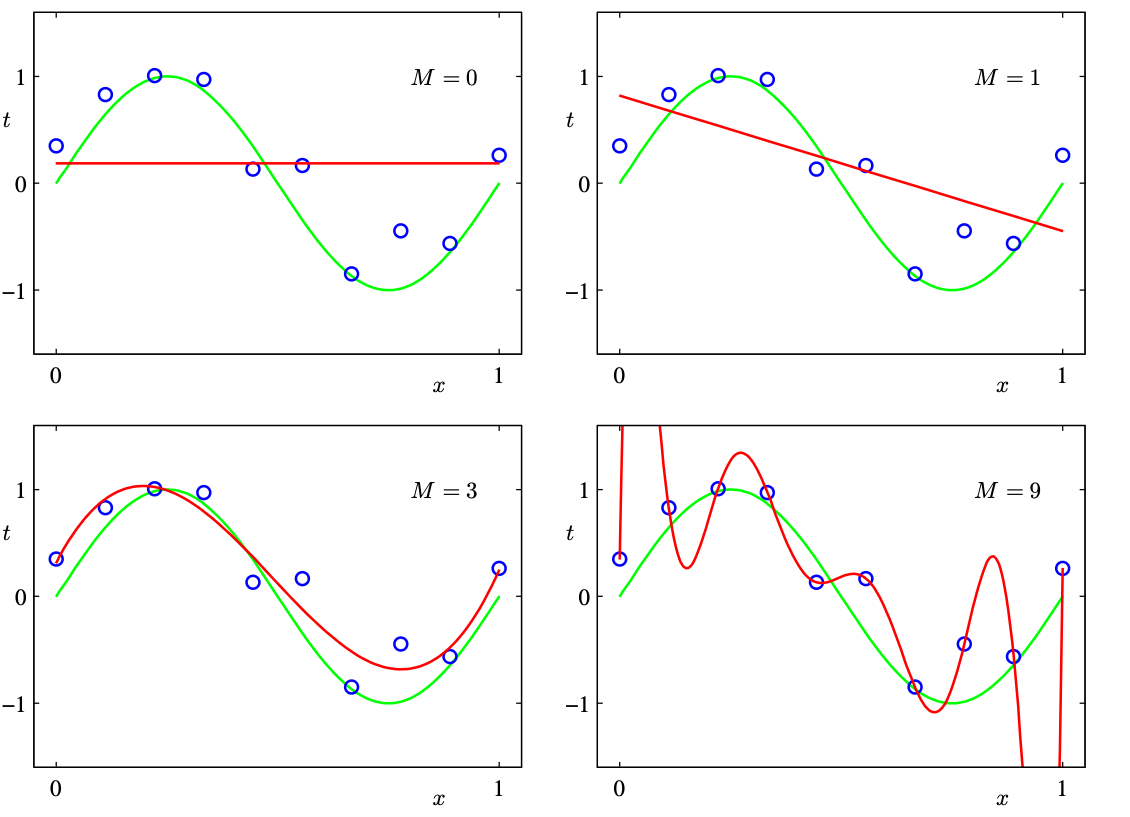
\includegraphics[scale=0.25]{chapter006/figures/fig002}
    \caption{handwritten digits}
    \label{handwritten digits}
\end{figure}

It is also interesting to examine the behavior of a given model as the size of the data set is varied. For a given model complexity, the over-fitting problem because less severe as the size of the data set increases.

It would seem more reasonable to choose the complexity of the model according to the complexity of the problem being solved.

\section{Regularization}

One technique that is often used to control the over-fitting phenomenon in such cases is that of $regularization$, which is involves adding a penalty term to the error function in order to discourage the coefficients from reaching large values.

\begin{equation}
    \tilde{E}(\pmb{w}) = \frac{1}{2}\sum_{n=1}^M \{y(x_n, \pmb{w}) - t_n \}^2 + \frac{\lambda}{2}||\pmb{w}||^2
\end{equation}

where $||\pmb{w}||^2 = \pmb{w}^T\pmb{w} = w_0^2 + w_1^2 + ... + w_M^2$, and the coefficient $\lambda$ governs the relative importance of the regularization term compared with the sum-of-squares error term. Reduces the value of the coefficients. In the context of neural networks, this approach is known as \textbf{weight decay}.

\section{Exercises}

\subsection{Exercise 1}

Consider the sum-of-squares error function given by \ref{Loss function} in which the function  $y(x, \pmb{w})$\ref{Polynomial}. Show that the coefficients $w=\{w_i\}$ that minimize this error function are given by the solution to the following set of linear equations

\begin{equation}
    \sum_{j=0}^M A_{ij}w_j = T_i
\end{equation}

where

\begin{equation}
    A_{ij} = \sum_{n=1}^N (x_n)^{i + j}
\end{equation}

and

\begin{equation}
    T_i = \sum_{n=1}^N (x_n)^it_n
\end{equation}

Here a suffix $i$ and $j$ denotes the index of a component, whereas $(x)^i$ denotes x raised to the power of $i$.

\subsubsection{Solution}

Loss function is

\begin{equation}
    E(\pmb{w}) = \frac{1}{2} \sum_{n=1}^M \{y(x_n, \pmb{w}) - t_n\}^2
\end{equation}

\begin{equation}
    \frac{\partial E(\pmb{w})}{\partial w_i} = \frac{\partial \sum_{n=1}^M \{y(x_n, \pmb{w}) - t_n\}}{\partial w_i} = \sum_{n=1}^M \frac{\partial \{y(x_n, \pmb{w}) - t_n \}}{\partial w_i}
\end{equation}

since,

\begin{equation}
    \frac{\partial \{y(x_n, \pmb{w}) - t_n \}}{\partial w_i} = \frac{\partial (w_0x_n^0 + ... + x_ix_n^i + ... + w_M x_n^M)}{\partial w_i} = x_n^i
\end{equation}

thus,


\begin{equation}
    \frac{\partial E(\pmb{w})}{\partial w_i} = \sum_{n=1}^M \{y(x_n, \pmb{w}) - t_n\} x_n^i
\end{equation}

\begin{equation}
    \frac{\partial E(\pmb{w})}{\partial w_i} = 0 \Leftrightarrow \sum_{n=1}^N \{y(x_n, \pmb{w}) - t_n\}x_n^i = 0 \Leftrightarrow \sum_{n=1}^N \{y(x_n, \pmb{w})x_n^i = \sum_{n=1}^N t_n x_n^i
\end{equation}

\begin{equation}
    \sum_{n=1}^N \{y(x_n, \pmb{w})x_n^i = \sum_{n=1}^N t_n x_n^i \Leftrightarrow \sum_{n=1}^N (\sum_{j=0}^M w_jx_n^j) x_n^i = \sum_{n=1}^N t_n x_n^i
\end{equation}

\begin{equation}
    \sum_{n=1}^N (\sum_{j=0}^M w_jx_n^j) x_n^i = \sum_{n=1}^N t_n x_n^i \Leftrightarrow \sum_{j=0}^M \sum_{n=1}^N (x_n^{(i + j)}w_j) = \sum_{n=1}^N t_nx_n^i
\end{equation}

Intuitively, given N = 2, M = 2

\begin{equation}
    \begin{split}
        \sum_{n=1}^N \sum_{j=0}^M (w_jx_n^i)x_n^i & = \sum_{n=1}^N (w_0x_n^0 + w_1x_n^1 + w_2x_n^2)x_n^i\\
        & = \sum_{n=1}^N (w_0x_n^0x_n^i + w_1x_n^1x_n^i + w_2x_n^2x_n^i)\\
        & = (w_0x_1^1x_1^i + w_1x_1^1x_1^i + w_2x_1^2x_1^i) + (w_0x_2^1x_2^i + w_1x_2^1x_2^i + w_2x_2^2x_2^i)\\
        & = \sum_{j=0}^M (w_jx_1^jx_1^i) + \sum_{j=0}^M (w_jx_2^jx_2^i)\\
        & = \sum_{j=0}^M (w_jx_1^{(i+j)}) + \sum_{j=0}^M (w_jx_2^{(i+j)})\\
        & = \sum_{j=0}^M \sum_{n=1}^N x_i^{(i + j)}w_j
    \end{split}    
\end{equation}


If $A_{ij} = \sum_{n=1}^N x_n^{(i + j)}$ and $T_i = \sum_{n=1}^N x_n^it_n$, then

\begin{equation}
    \sum_{j=0}^M A_{ij}w_j = T_i
\end{equation}


\subsection{Exercise 2}

Similar to the exercise 1, but now apply to the loss function

\begin{equation}
    E(\pmb{w}) = \frac{1}{2} \sum_{n=1}^M \{y(x_n, \pmb{w}) - t_n\}^2 +  \frac{\lambda}{2} ||w_i||^2
\end{equation}

since $||w_i||^2 = w_i^2 $, we have

\begin{equation}
    \frac{\partial E(\pmb{w})}{\partial w_i} = \sum_{n=1}^N \{y(x_n, \pmb{w}) - t_n\} x_n^i + \lambda w_i = \sum_{n=1}^N \{y(x_n, \pmb{w})x_n^i - \sum_{n=1}^N t_nx_n^i + \lambda w_i
\end{equation}

\begin{equation}
    \frac{\partial E(\pmb{w})}{\partial w_i} = 0 \Leftrightarrow \sum_{n=1}^N \{y(x_n, \pmb{w})x_n^i + \lambda w_i = \sum_{n=1}^N t_n x_n^i 
\end{equation}


\begin{equation}
    \frac{\partial E(\pmb{w})}{\partial w_i} = 0 \Leftrightarrow \sum_{j=0}^M (\sum_{n=1}^N x_n^{(i + j)}w_j) + \lambda w_i = \sum_{n=1}^N t_n x_n^i 
\end{equation}

Intuitively, given $M = 2$ and $N = 2$, then $\sum_{j=0}^M \sum_{n=1}^N (x_n^{(i + j)})w_j + \lambda w_i$ equals

\begin{equation}
    \begin{split}
        & = \sum_{j=0}^M (x_1^{(i + j)} + x_2^{(i + j)})w_j + \lambda w_i\\
        & = (x_1^{(i + j)} + x_2^{(i + j)})w_0 + (x_1^{(i + j)} + x_2^{(i + j)})w_1 + (x_1^{(i + j)} + x_2^{(i + j)})w_2 + \lambda w_i
    \end{split}
\end{equation}

since $0 \leq i \leq M$, if $i=1$, then 

\begin{equation}
    \begin{split}
        & = (x_1^{(i + j)} + x_2^{(i + j)})w_0 + (x_1^{(i + j)} + x_2^{(i + j)})w_1 + (x_1^{(i + j)} + x_2^{(i + j)})w_2 + \lambda w_1\\
        & = (x_1^{(i + j)} + x_2^{(i + j)})w_0 + (x_1^{(i + j)} + x_2^{(i + j)} + \lambda)w_1 + (x_1^{(i + j)} + x_2^{(i + j)})w_2\\
        & = (x_1^{(i + j)} + x_2^{(i + j)} + \delta \lambda)w_0 + (x_1^{(i + j)} + x_2^{(i + j)} + \delta \lambda)w_1 + (x_1^{(i + j)} + x_2^{(i + j)} + \delta \lambda)w_2
    \end{split}
\end{equation}

where $\delta = 0$ if $i \neq j$, otherwise $\delta = 1$. So

 \begin{equation}
     \begin{split}
         \sum_{j=0}^M (\sum_{n=1}^N x_n^{(i + j)}w_j) + \lambda w_i = \sum_{j=0}^M (\sum_{n=1}^N x_n^{(i + j)}w_j + \delta \lambda)
     \end{split}
 \end{equation}
 
 or
 
 \begin{equation}
     \frac{\partial E(\pmb{w})}{\partial w_i} = 0 \Leftrightarrow \sum_{j=0}^M (\sum_{n=1}^N x_n^{(i + j)}w_j + \delta \lambda) = \sum_{n=1}^N t_n x_n^i
 \end{equation}